\textit{This secion will go in depth with the extension-board created as an addon to the AQ M4 board. The extension-board was developed to act as a bridge between the PC and the CAN-bus using wireless communication.} \\

\subsubsection*{Wireless communication module} \label{sec:wireless_communication_module}
An important part of the hardware is the wireless communication used between the PC and the drones.
The wireless communication module has several requirements it needs to fulfill in order to make the whole system work as expected. A comparison table has been made in table \ref{tab:compare_table_wireless_communication} to find the wireless communication module that is best suited for the task. \\

A description of the modules compared can be seen in appendix \ref{app:wireless_decribe}

\begin{savenotes}
\begin{table}[H]
	\centering
	\resizebox{\textwidth}{!}{%
	\begin{tabular}{@{}|l|l|l|l|l|l|l|l|@{}}
		\toprule
		\textbf{Product} & \textbf{Size} & \textbf{Weight} & \textbf{Price} & \textbf{Documentation} &  \textbf{Range}  & \textbf{Score} \\ \midrule
		ESP8266   &  24x16mm\footnote{\url{https://www.mikrocontroller.net/attachment/243558/fcc\_11.pdf} last visited 26 Maj} \hfill\{7\} & 1.5g\footnote{Measured by author on chemistry weight} \hfill\{8\} &   7.5\$\footnote{\url{http://www.seeedstudio.com/depot/ESP8266-based-WiFi-module-SPI-supported-p-2486.html} last visited 26 Maj}  \hfill\{9\}  &   Great community \hfill\{9\}  &    ?    &          33      		\\ \midrule
		EMW3165   &  32x16mm\footnote{\url{https://hackadaycom.files.wordpress.com/2015/07/emw3165.pdf} last visited 26 Maj} \hfill\{6\}  & 5g\footnote{\url{http://www.seeedstudio.com/depot/EMW3165-CortexM4-based-WiFi-SoC-Module-p-2488.html} last visited 26 Maj} \hfill\{2\} &  9\$\footnote{\url{http://www.seeedstudio.com/depot/EMW3165-CortexM4-based-WiFi-SoC-Module-p-2488.html}} \hfill\{8\}   &  Less available  \hfill\{3\}	        &    ?    &    19            		\\ \midrule
		nRF51822  &  18x10mm\footnote{\url{http://www.fanstel.com/Product/bluenor.html}last visited 26 Maj} \hfill\{8\}  & 3g\footnote{\url{http://www.seeedstudio.com/depot/MDBT40P\%C2\%A0\%C2\%A0nRF51822\%C2\%A0based\%C2\%A0BLE\%C2\%A0module-p-2503.html} last visited 26 Maj} \hfill\{4\}  &  7.5\$ \footnote{\url{http://www.seeedstudio.com/item_detail.html?p_id=2503} last visited 26 Maj} \hfill\{9\}   & Ok documented\hfill\{2\} 	        &   30 M\footnote{\url{https://dl.dropboxusercontent.com/u/54939426/Fanstel_BT600.pdf} last visited 26 Maj}  \hfill\{9\}     &               32 		\\ \midrule
		XBee      &  24.38x27.61mm \footnote{\url{http://www.digi.com/products/xbee-rf-solutions/modules/xbee-802-15-4\#specifications}} \{3\} & 3g \footnote{\url{http://www.digi.com/products/xbee-rf-solutions/modules/xbee-802-15-4\#specifications} last visited 26 Maj} \hfill\{4\} &   25\$\footnote{\url{https://www.sparkfun.com/products/11215} last visited 26 Maj}  \hfill\{4\}  &  Lots of DIY   \hfill\{9\}      &            91 M\footnote{\url{https://www.sparkfun.com/pages/xbee_guide}}  \hfill\{9\}  &             29       \\ \bottomrule
	\end{tabular}}
	\caption{Comparisontable used to compare different wireless 		communication modules}
	\label{tab:compare_table_wireless_communication}
\end{table}
    \end{savenotes}

The products compared in \ref{tab:compare_table_wireless_communication} are chosen to have approximately same specs such as onboard antenna and no need for extra components.
The ESP8266 module based on the highest score but must of all because it is use in a wide range of applications and has a lot of activity on their official Arduino github. The weight of the module was measured after the decision was made. If it was heavier than the other modules it would still have been used due to the large number of projects using this module. In case help was needed to make the module work, plenty of projects is available online and they have an active forum\footnote{\url{http://www.esp8266.com/} last visited 26 Maj}

\subsubsection*{Microcontroller}
The list below shows the requirement for the microcontroller on the extension-board.
\begin{itemize}
	\item \textbf{CAN-controller} to communicate with the AQ M4 board.
	\item \textbf{2 UART} to communicate with the ESP8266-module and with a PC for debugging purpose.
	\item \textbf{Small package} such as QFN64 (9*9mm)
\end{itemize}

The AT90CAN128 was chosen since the author and SDU had experience programming and using that microcontroller. It meets the requirements as well since it has built-in CAN controller,  two UARTS and is available in QFN64 package.
Kjeld Jensen has been in front of the development of the Frobomind-controller\footnote{\url{http://www.frobomind.org/index.php/FMCtrl:FroboMind\_Controller} last visited 22 Maj}, which uses the AT90CAN128 microcontroller.
Since the Frobomind-controller was available the author could start developing the firmware while the PCB for the ladybirds were made.

\subsubsection*{Block Schematic}
The block schematic shown in figure \ref{fig:PCB_block} was created by the author. It was then given to Carsten Albertsen who created the schematic and did rest of the creation of the PCB. Some time was spend  debugging since there was an error in the ISP pins. Later on the author had to make a correction to the board since a pin(GPIO15) on the ESP8266 that had to be grounded in order to select booting from the flash.
\begin{figure}[H]
    \center
    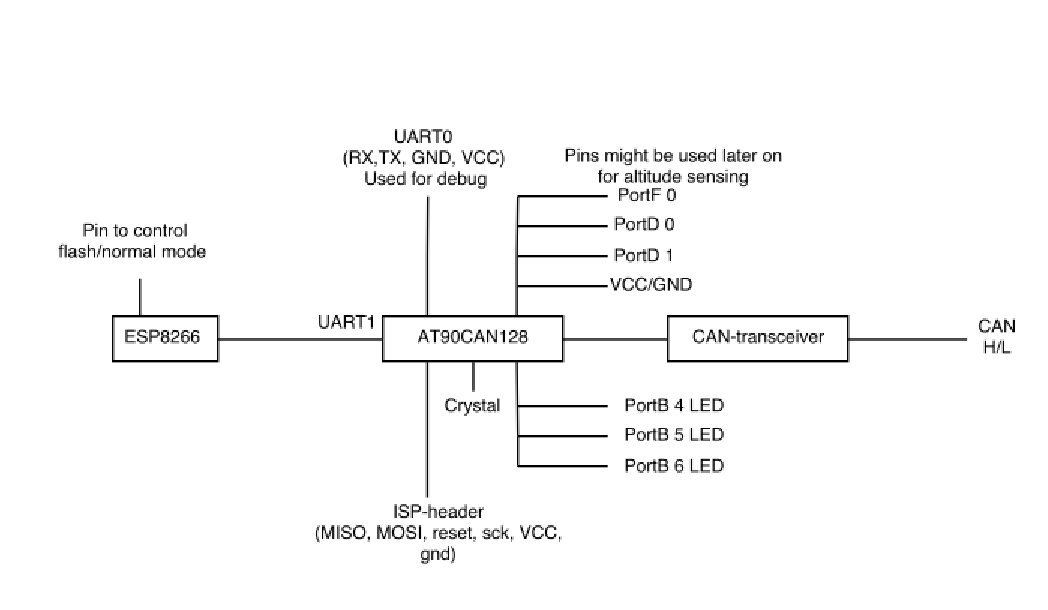
\includegraphics[width=0.9\textwidth]{graphics/PCB_block_v3.eps}
    \caption{Block schematic of the extension-board developed to AQ M4. It can be seen that the ESP8266 chip is connected to the At90CAN128 using UART1 and that the At90CAN128 is connected to a CAN-transceiver.}
    \label{fig:PCB_block}
\end{figure}

\subsubsection*{Pins}
A few pins where made available through solder pads for easy access if needed later on.

The following pins where available as solder pads:
\begin{itemize}
	\item PortF 0 - Alternative function as ADC, channel 0
	\item PortD 0 - Alternative function as interrupt, INT0 and I2C, SCL
	\item PortD 1 - Alternative function as interrupt, INT1 and I2C, SDA
\end{itemize}
In case the onboard barometer is not accurate enough to keep the drone at a constant height, an alternative distance could be used to measure the drones altitude with respect to the ground.
PortF0 has been made available since some distance sensors give output as an analogue value. 
An example of such sensor is an Infrared proximity sensor.\footnote{\url{http://www.sharpsma.com/webfm\_send/1208}} \\
As an alternative type of distance sensor, a ultrasoinc could be used such as HCSR04.
As output it gives a binary output with high-time proportional with the distance.\footnote{\url{http://www.micropik.com/PDF/HCSR04.pdf}}.
To detect the high-time, one of PortD1/0 would be useful.
Sensors using I2C could be used as well.\\
Which type of sensor suits best as a distance sensor to provide altitude information to the drone is ouf of scope of this report. The PCB has just been made ready to support different types of sensors.

\subsubsection*{Debug/ISP}
In the final schematic \ac{UART}0 and ISP pins where combined in one pinheader for easy access through one cable.
The connector can be seen in figure \ref{fig:extension_board}.

To program the At90CAN128 the ISP pins where required to be easy accessable. 
\ac{UART}0 was made accessable to be used as debug and programming of the ESP8266 board.
The idea was to setup the At90CAN128 as \ac{UART} passthrough from \ac{UART}0 to \ac{UART}1.
Due to a mistake \footnote{The wrong pair of MISO/MOSI pins where made available in the ISP-header. The correct pair of MISO/MOSI is also RXD0/TXD0 as alternative function} in the final schematic\footnote{Can be found at \textit{Appendix/ESP8266\_CAN\_Autoquad29032016\_3.PDF}}, both \ac{UART}0 and \ac{UART}1 where made accessible trough the ISP/debug header. 
This ended up making it easier to program the ESP8266-board without using the At90CAN128 as \ac{UART} pass-through.

\begin{figure}[H]
    \centering
    \begin{subfigure}[b]{0.45\textwidth}
        \includegraphics[width=\textwidth]{graphics/extension_board_up}
        \caption{Top-view of the developed extension-board. If looking carefully, the ISP-fix can be seen between the ESP-8266 module and the Debug/ISP pins.}
        \label{fig:extension_board_up}
    \end{subfigure}
    ~ 
    \begin{subfigure}[b]{0.51\textwidth}
        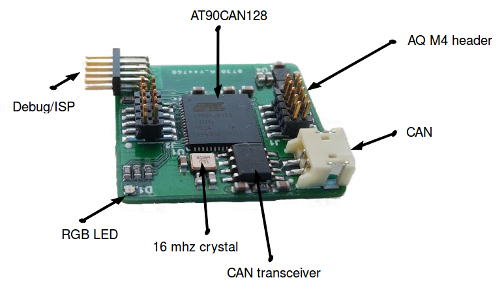
\includegraphics[width=\textwidth]{graphics/extension_board_down}
        \caption{Bottom-view of the developed-extension board. The two connects for the AQ M4 board can be seen pointing up. The CAN-connect is of same type mounted on the AQ M4 board.}
        \label{fig:extension_board_down}
    \end{subfigure}
    \caption{Top and bottom view of the extension-board}\label{fig:extension_board}
\end{figure}

Test of the extension-board was done by making small sketches testing the individual parts of the circuit. The sketches used to blink the leds and proof that the basic functionality works is left out. CAN is tested in section \ref{sec:test_of_queues}.

\subsubsection*{Test of WIFI range}
Two tests were conducted in order to see how the latency and range behaves when the distance is increased.
The firmware of the ESP8266 module had to be flashed to specify which access point \footnote{The network configuration is described in section \ref{sec:network_configuration}} it should connect to.
The test was conducted by increasing the distance between the ESP8266 module and the laptop by 1 meter. 

After each distance increase, the laptop pinged the ESP8266 module 200 times with 10 hz with a packet size equal to the size of the frame used.
\footnote{The WIFI frame is described in section \ref{sec:system_architecture_indoor}}.
The tests were conducted on an open grass field in order to avoid as much disturbance as possible.
 
Figure \ref{fig:wifi_pingtest} shows the results of the ping test.

\begin{figure}[H]
    \center
    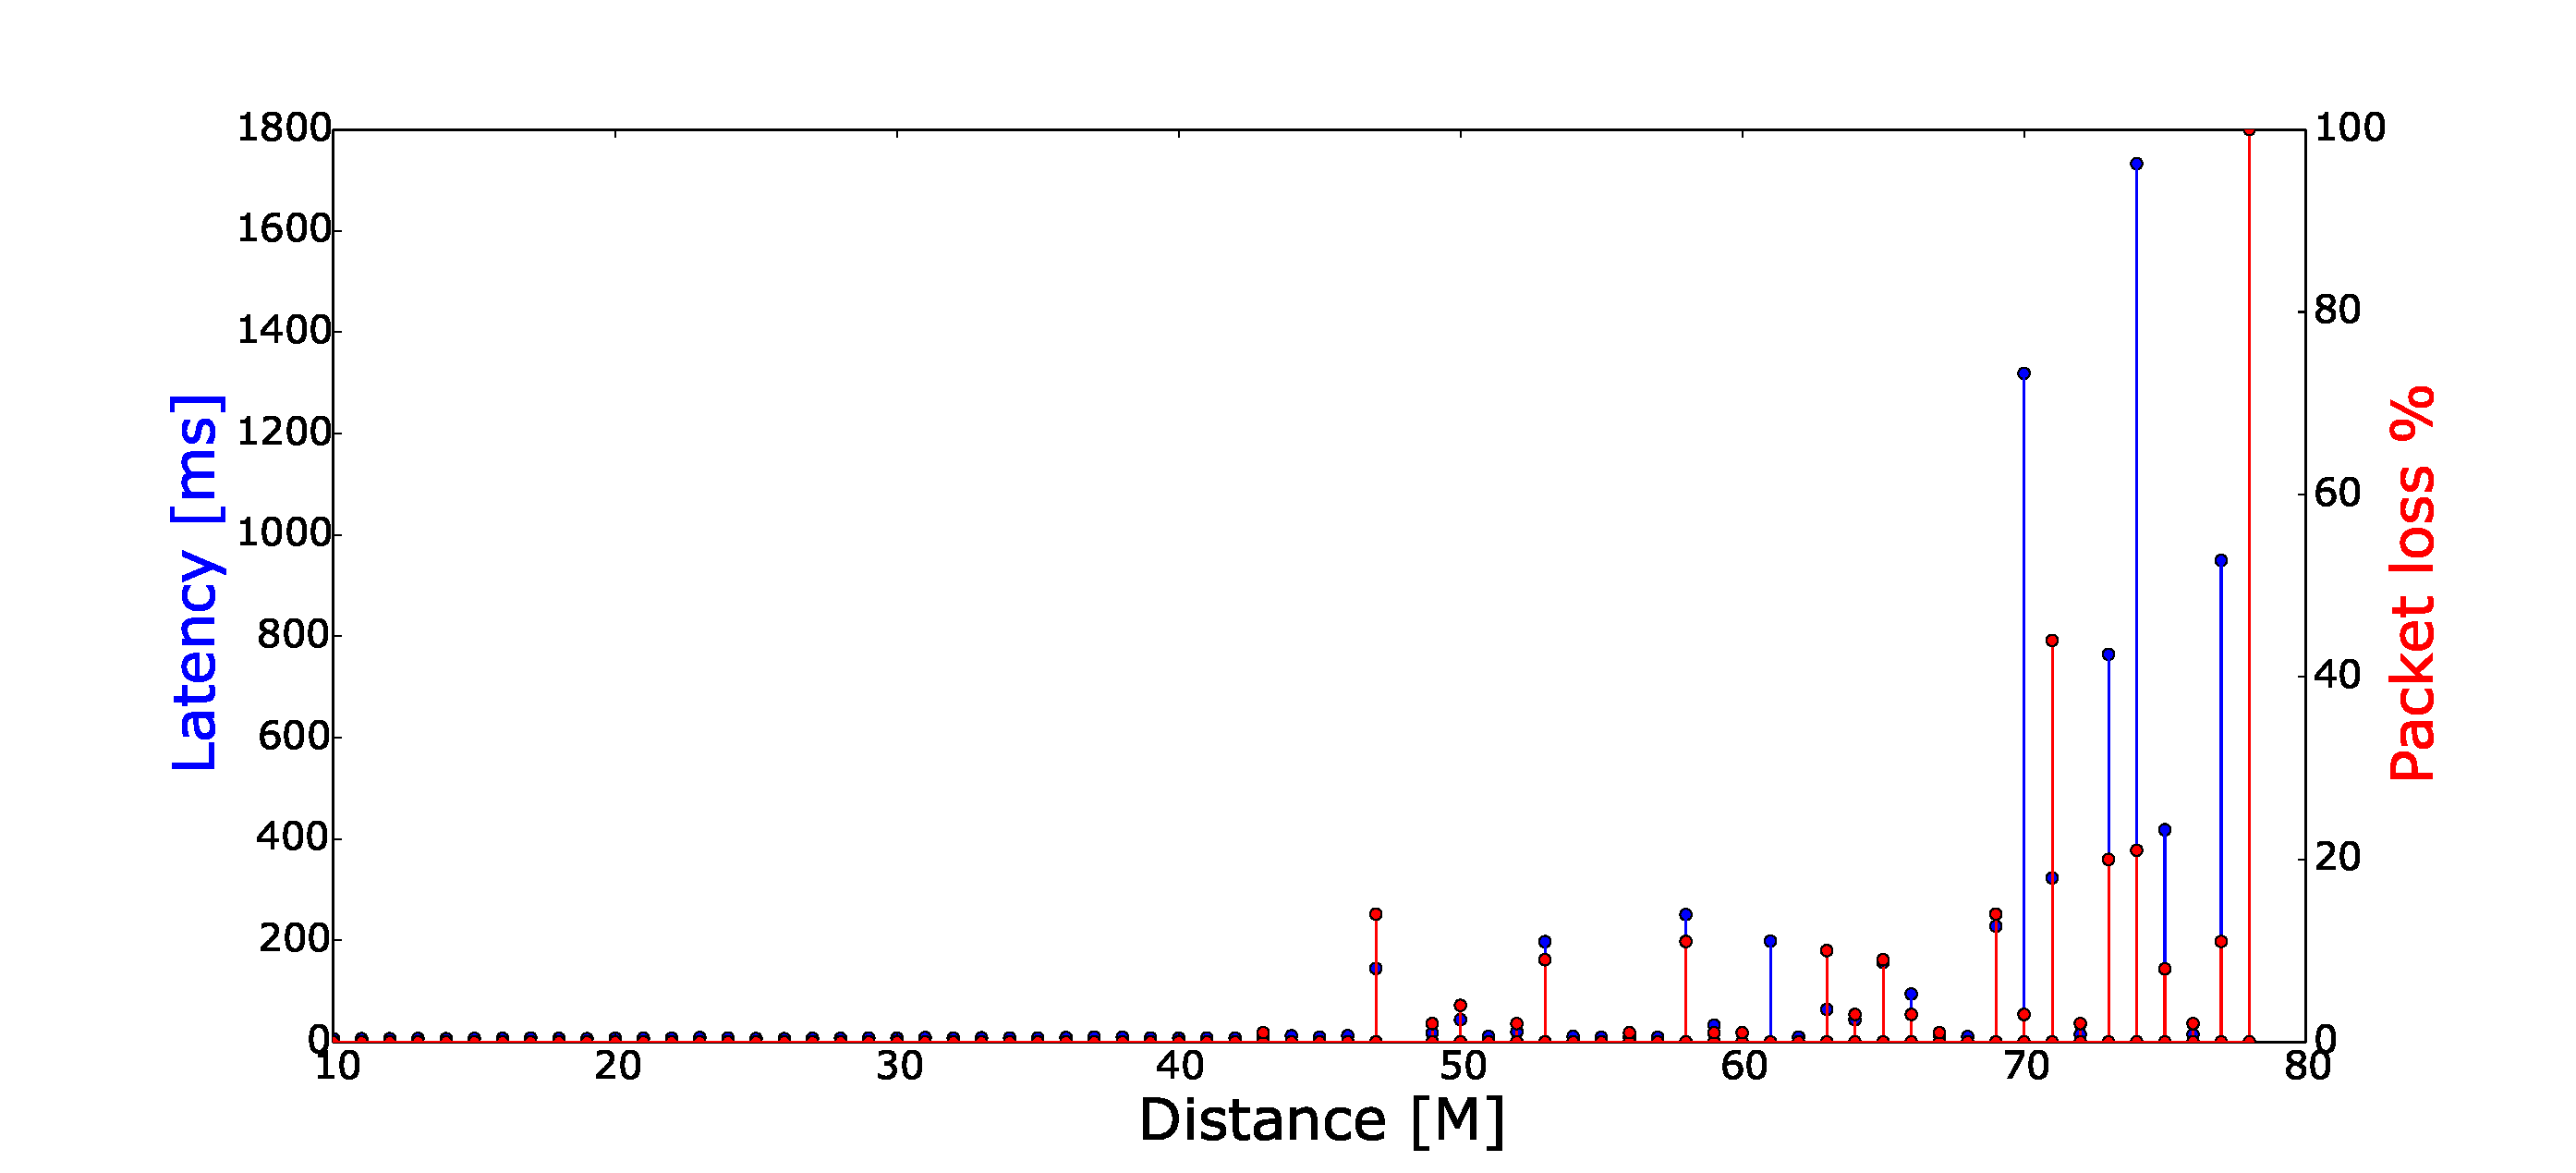
\includegraphics[width=0.9\textwidth]{graphics/wifi_test_latency_1.eps}
  \caption{Plot shows the average latency, packet loss vs. distance. Up until 46 meters no packets are dropped and the latency is quite low.}
    \label{fig:wifi_pingtest}
\end{figure}

It can be seen, that until 46 Meters no packets is dropped and the latency is low. From 46 to 69 the latency starts to increase and packets begin to get dropped. At 69 meters and up to 80 meters the latency is high and packet loss percentage is increased. Since ping works by sending a request and waiting for the answer this tests communication both ways. However only one way communication from the laptop to the ESP8266 is required.


The purpose of a second test was to see what happens with the number of valid CRC\footnote{CRC described in section \ref{sec:extension_board_firmware}} frames\footnote{Frame described in section \ref{sec:system_architecture_indoor}} as the distance is increased.
The distance was increased by 1 meter in the beginning, however to save time it was increased to 5 meters and later 10 meters. 
When the module started to miss frames or CRC was not verified the distance between tests went down to 5 meter again.

Figure \ref{fig:wifi_crc_check} shows the result.

\begin{figure}[H]
    \center
    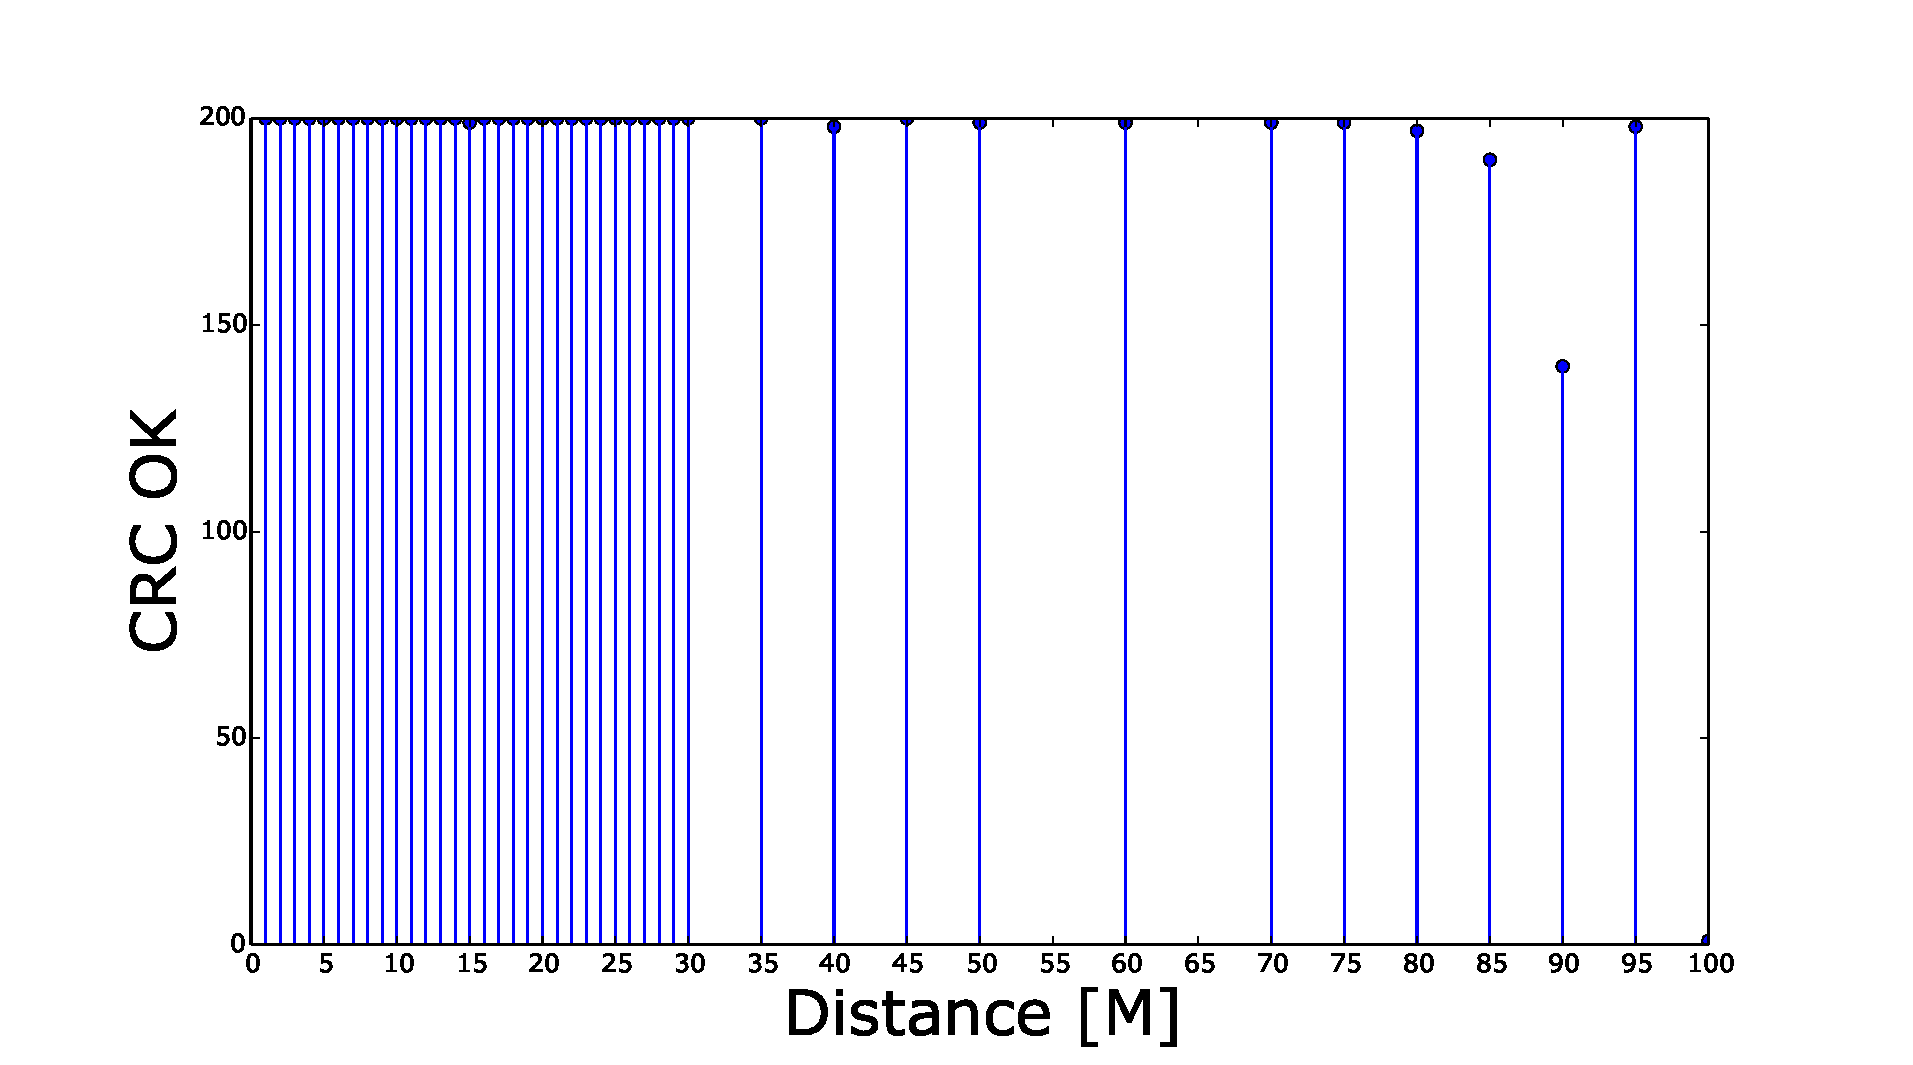
\includegraphics[width=0.85\textwidth]{graphics/crc_distance_check.eps}
	\caption{Measurements was initially done at every meter, however to save time the distance was increase to 5 meter and later to 10. When packets began to drop, measurements was done at 5 meter interval again. At 100 meters the WIFI connection was dropped.}
    \label{fig:wifi_crc_check}
\end{figure}

At figure \ref{fig:wifi_pingtest} and \ref{fig:wifi_crc_check} it can be seen, that at a distance higher than 46 meters the latency increases but almost every CRC packet is received and valid. At 90 meters the number of valid frames drops and a ping response is not received. Even though frames it still received and valid they will be delayed.


A final test was made to see how the modules behave when two modules are receiving the packets. At 10 hz 200 frames were sent to two modules at a distance of 10 meters.
Unfortunately only one connector to communicate with the extension-board were made which made it difficult to check if both extension-boards received the data without error at the same time. The test was done 4 times while alternating between the modules to verify both modules were receiving all the packets.\footnote{If more time were available, a timing-test of the setup would have been done. By measuring the time it takes one drones to receive 200 packets, do the same test but when two drones each receiving 200 packets.}
\begin{figure}[H]
    \centering
        \includegraphics[width=0.5\textwidth]{graphics/laptop_extenbioard_crc_check}
        \caption{Test setup where two modules receives 200 frames at 10 hz at the same time. It can be seen that the laptop only checks the received number of frames one extension-board at a time.}
        \label{fig:crc_distance_check}
\end{figure}
Both modules received 200 packets without CRC error 

\subsubsection*{Conclusion}
It can be concluded that the ESP8266 wireless module was chosen based on requirements in table \ref{tab:compare_table_wireless_communication}. The ESP8266 got the highest score and was mainly chosen since it is a widely used module. The extension-board was created based on the block schematic shown in figure \ref{fig:PCB_block}. A At90CAN128 was chosen based on its build-in CAN-controller, it was avilable and it because of previous experience. Three tests was conducted to test the performance of ESP8266 module. If the distance is larger than 46 meters the latency begins to increase and the CRC packets will be arrive without error but will delayed. If the distance is larger than 85 meters the packets suffers from high latency and errors starts to occur.
At a distance of 70 meters packets experience latency up to 1.4 sec. If a frame containing a drones positions arrives 1.4 sec too late it is invalid since the drone could have moved several meters since the frame was sent.

